% !TEX encoding = UTF-8
% !TEX program = pdflatex
% !TEX root = AALP.tex
% !TEX spellcheck = it-IT
\documentclass[a4paper, 11pt]{report} % Font size (can be 10pt, 11pt or 12pt) and paper size (remove a4paper for US letter paper)
\usepackage[italian]{babel}      							% Lingua italiana
\usepackage[margin=.9in]{geometry}             % Imposta i margini del documento

\usepackage[T1]{fontenc} % Required for accented characters
\usepackage[mathletters]{ucs}    % Caratteri matematici come UTF8
\usepackage[utf8,utf8x]{inputenc}      % Ancora utf8

\usepackage{eurosym}                %simbolo dell'euro
\usepackage{listings}
\usepackage[usenames,dvipsnames,svgnames,table]{xcolor}
% Imposta lo spazio nella list of listing in modo simile alla list of figures/tables
%\makeatletter
%\let\my@chapter\@chapter
%\renewcommand*{\@chapter}{%
%  \addtocontents{lol}{\protect\addvspace{10pt}}%
%  \my@chapter}
%\makeatother


\definecolor{codegreen}{rgb}{0,0.6,0}
\definecolor{codegray}{rgb}{0.5,0.5,0.5}
\definecolor{backcolor}{rgb}{0.98,0.98,0.98}

\renewcommand{\lstlistingname}{Codice}% Listing -> codice
\renewcommand{\lstlistlistingname}{Elenco dei frammenti di codice}% List of Listings -> Frammenti di codice

\lstdefinestyle{mystyle}{
    backgroundcolor=\color{backcolor},   
    commentstyle=\color{Peach}\ttfamily,
    keywordstyle=\color{RoyalBlue},
    numberstyle=\tiny\color{codegray},
    stringstyle=\color{SeaGreen}\ttfamily,
    basicstyle=\footnotesize\ttfamily,
    breakatwhitespace=false,         
    breaklines=true,                 
    captionpos=b,                    
    keepspaces=true,                 
    numbers=left,                    
    numbersep=5pt,                  
    showspaces=false,                
    showstringspaces=false,
    showtabs=false,                  
    tabsize=2,
    frame=trbl, % draw a frame at the top, right, left and bottom of the listing
	frameround=ftff, % angolo in basso a destro curvo
	framesep=4pt, % quarter circle size of the round corners,
	inputencoding=utf8,
    extendedchars=true,
    literate={á}{{\'a}}1 {à}{{\`a}}1 {é}{{\'e}}1 {è}{{\`e}}1 {ù}{{\`u}}1 {ò}{{\`o}}1 {ì}{{\`i}}1,
    belowskip=1em,
    aboveskip=1em,
}

 
\lstset{style=mystyle}

\lstdefinelanguage{JavaScript}
{
  % list of keywords
  morekeywords={ true, false, catch, function, break,	new, class, extends, var, require, switch, return, import, if, while, for, this, View, Text, StyleSheet},
  sensitive=false, % keywords are not case-sensitive
  morecomment=[l]{//}, % l is for line comment
  morecomment=[s]{/*}{*/}, % s is for start and end delimiter
  morestring=[b]' % defines that strings are enclosed in double quotes
}

\lstdefinelanguage{JSON}
{
  % list of keywords
  morekeywords={string, boolean, int, Array, Node, Asset, AssetDetail, Filter, FilterItem},
  sensitive=false, % keywords are not case-sensitive
  morecomment=[l]{//}, % l is for line comment
  morecomment=[s]{/*}{*/}, % s is for start and end delimiter
  morestring=[b]" % defines that strings are enclosed in double quotes
}

\lstdefinelanguage{URM}
{
	% list of keywords
	morekeywords={ S, J, T, Z, I},
	sensitive=false, % keywords are not case-sensitive
	morecomment=[l]{//}, % l is for line comment
	morecomment=[s]{/*}{*/}, % s is for start and end delimiter
	morestring=[b]' % defines that strings are enclosed in double quotes
}

\lstdefinelanguage{RDFA}{
	language=html,
	sensitive=true, 
	alsoletter={<>=-},
	ndkeywords={
		% General
		=,
		% HTML attributes
		charset=, id=, width=, height=, property=, about=, rel=, rev=, prefix=, vocab=, content=, datatype=
	},  
	morecomment=[s]{<!--}{-->},
	tag=[s]
}

%\tightlist per compatibilità con pandoc
\providecommand{\tightlist}{%
	\setlength{\itemsep}{0pt}\setlength{\parskip}{0pt}}


\usepackage[labelfont=bf]{caption}

\usepackage[protrusion=true,expansion=true]{microtype} % Better typography
\usepackage{graphicx} % Required for including pictures
\usepackage{wrapfig} % Allows in-line images


\usepackage{subfig}
\usepackage{hyperref}
\usepackage{placeins}
\usepackage{sourcecodepro}
\usepackage{hyperref}                   % collegamenti ipertestuali

\usepackage[colorinlistoftodos,prependcaption]{todonotes} %todo

\usepackage{amsmath}
\usepackage{mathtools}

\usepackage{float}
\usepackage{algorithm}
\usepackage{algpseudocode} % https://en.wikibooks.org/wiki/LaTeX/Algorithms#Typesetting_using_the_algorithmicx_package
\usepackage{amssymb}  %$\mathbb{N}$ per il simbolo dei numeri naturali 

\usepackage{enumerate} % permette di personalizzare enumerate

\usepackage{xmpincl}	%Aggiunge metadati sulla licenza CC
\usepackage{xspace}
\makeatletter
\renewcommand\@biblabel[1]{\textbf{#1.}} % Change the square brackets for each bibliography item from '[1]' to '1.'
\renewcommand{\@listI}{\itemsep=0pt} % Reduce the space between items in the itemize and enumerate environments and the bibliography

\renewcommand{\maketitle}{ % Customize the title - do not edit title and author name here, see the TITLE block below
	\begin{flushright} % Right align
		{\LARGE\@title} % Increase the font size of the title
		
		\vspace{50pt} % Some vertical space between the title and author name
		
		{\large\@author} % Author name
		\\\@date % Date
		
		\vspace{100pt} % Some vertical space between the author block and abstract
	\end{flushright}
}

%% breakablealgorithm http://tex.stackexchange.com/questions/33866/algorithm-tag-and-page-break
\makeatletter
\newenvironment{breakablealgorithm}
{% \begin{breakablealgorithm}
	\begin{center}
		\refstepcounter{algorithm}% New algorithm
		\hrule height.8pt depth0pt \kern2pt% \@fs@pre for \@fs@ruled
		\renewcommand{\caption}[2][\relax]{% Make a new \caption
			{\raggedright\textbf{\ALG@name~\thealgorithm} ##2\par}%
			\ifx\relax##1\relax % #1 is \relax
			\addcontentsline{loa}{algorithm}{\protect\numberline{\thealgorithm}##2}%
			\else % #1 is not \relax
			\addcontentsline{loa}{algorithm}{\protect\numberline{\thealgorithm}##1}%
			\fi
			\kern2pt\hrule\kern2pt
		}
	}{% \end{breakablealgorithm}
	\kern2pt\hrule\relax% \@fs@post for \@fs@ruled
\end{center}
}
\makeatother

\makeatletter % trattino con punto sopra
\newcommand{\dotminus}{\mathbin{\text{\@dotminus}}}

\newcommand{\@dotminus}{%
	\ooalign{\hidewidth\raise1ex\hbox{.}\hidewidth\cr$\m@th-$\cr}%
}
\makeatother

\DeclarePairedDelimiter{\ceil}{\lceil}{\rceil}
\DeclarePairedDelimiter{\floor}{\lfloor}{\rfloor}

\newcommand{\false}{\text{ false }}
\newcommand{\true}{\text{ true }}
\newcommand{\fn}{\text{fn }}
\newcommand{\iif}{\text{ if }}
\newcommand{\then}{\text{ then }}
\newcommand{\eelse}{\text{ else }}
%----------------------------------------------------------------------------------------
% TITLE
%----------------------------------------------------------------------------------------

\title{\textbf{Aspetti Avanzati dei Linguaggi di Programmazione}\\ % Title
	A.A. 2016-2017 } % Subtitle

\author{\textsc{Giacomo Manzoli}
	\\ 1130822 % Author
	\\{\textit{Università degli Studi di Padova}}} % Institution

\date{\today} % Date

%----------------------------------------------------------------------------------------


%----------------------------------------------------------------------------------------
%	DOCUMENT HEADER
%----------------------------------------------------------------------------------------

\begin{document}
	
	\maketitle % Print the title section

	%----------------------------------------------------------------------------------------
	% ABSTRACT AND KEYWORDS
	%----------------------------------------------------------------------------------------
	
	%\renewcommand{\abstractname}{Summary} % Uncomment to change the name of the abstract to something else
	
	\clearpage
	\tableofcontents
	
	%\hspace*{3,6mm}\textit{Keywords:} lorem , ipsum , dolor , sit amet , lectus % Keywords
	
	\vspace{30pt} % Some vertical space between the abstract and first section
	
	%----------------------------------------------------------------------------------------
	% ESSAY BODY
	%----------------------------------------------------------------------------------------
	\clearpage
	
	%----------------------------------------------------------------------------------------
	%	CONTENT
	%----------------------------------------------------------------------------------------
	
	% !TEX encoding = UTF-8
% !TEX TS-program = pdflatex
% !TEX root = computabilità e algoritmi.tex
% !TEX spellcheck = it-IT
\chapter{Funzioni calcolabili e Modelli di calcolo}
\section{Introduzione}\label{lezione-1---computabilituxe0-e-algoritmi}

Ci sono dei problemi che non possono essere risolti in modo algoritmico,
come la terminazione o la prova di correttezza di un programma, lo studio di questi problemi prende il nome di teoria della computabilità.

In questa teoria non viene preso in considerazione il consumo di
risorse in modo che le dimostrazioni effettuate siano indipendenti dal
modello di calcolo adottato.

Notoriamente, i problemi appartengono a varie classi di difficoltà:

\begin{itemize}
\item
  \textbf{P}: problemi che possono essere risolti da un algoritmo in
  tempo polinomiale
\item
  \textbf{NP}: problemi che possono essere risolti in tempo polinomiale
  ma in modo non deterministico
\item
  \textbf{EXP}: problemi che possono essere risolti da un algoritmo in
  tempo esponenziale
\end{itemize}

\subsection{L'informatica e la computabilità}\label{linformatica-e-la-computabilituxe0}

\emph{Computer science is no more about computers tha astronomy is about
telescopes. Dijkstra}.

L'idea dell'informatica nasce dalla logica, ricercando un procedimento
generale (macchina) su base combinatoria per trovare tutte le verità.

Libro: \emph{Nigel Cutland ``Computability. An Introduction to Recursive
Function Theory'' Cambridge University Press}.

	% !TEX encoding = UTF-8
% !TEX TS-program = pdflatex
% !TEX root = computabilità e algoritmi.tex
% !TEX spellcheck = it-IT
\chapter{Lezione 2}
\section{Introduzione e Algoritmi sui grafi}\label{lezione-2---introduzione-e-algoritmi-sui-grafi}

C'è la possibilità di fare un pre-orale nella settimana dei compitini.

Libro: Cormen, Introduzione agli algoritmi e strutture dati
\href{http://catalogo.unipd.it/F/FCKK1DACESL2TDH5CF15FLDL2BUM936U1XG9U15MFDCKI764BV-10675?func=full-set-set\&set_number=011139\&set_entry=000001\&format=999}{BIB}:

\begin{itemize}
\item
  Introduzione agli algoritmi sui grafi
  \begin{itemize}
  \item
    Strutture dati per i grafi
  \item
    Operazioni elementari sui grafi
  \end{itemize}
\item
  Algoritmi su stringhe (capitolo 22)
\item
  Algoritmi paralleli (capitolo 27)
\item
  Algoritmi di geometria computazionale
\end{itemize}

\subsection{Terminologia dei grafi}\label{terminologia-dei-grafi}

Un grafo \emph{G} è costituito da un insieme di vertici \emph{V} e di
archi \emph{E}. Ad ogni arco vengono associati due vertici in \emph{V}.

Se c'è un ordine tra i due estremi degli archi, il grafo prende il nome
di \textbf{orientato} o \textbf{diretto}. In questo caso, il primo
vertice prende il nome di \textbf{coda} e l'ultimo \textbf{testa}.

Un \textbf{cappio} è un arco i cui due estremi coincidono.

Un grafo non orientato si dice \textbf{semplice} se non ha cappi e non
ci sono due archi con gli stessi estremi. Mentre se il grafo è
orientato, perché sia semplice non devono esserci archi con gli stessi
estremi, iniziali e finali. Un grafo non semplice prende il nome di
\textbf{multi-grafo}.

\begin{figure}[htbp]
\centering
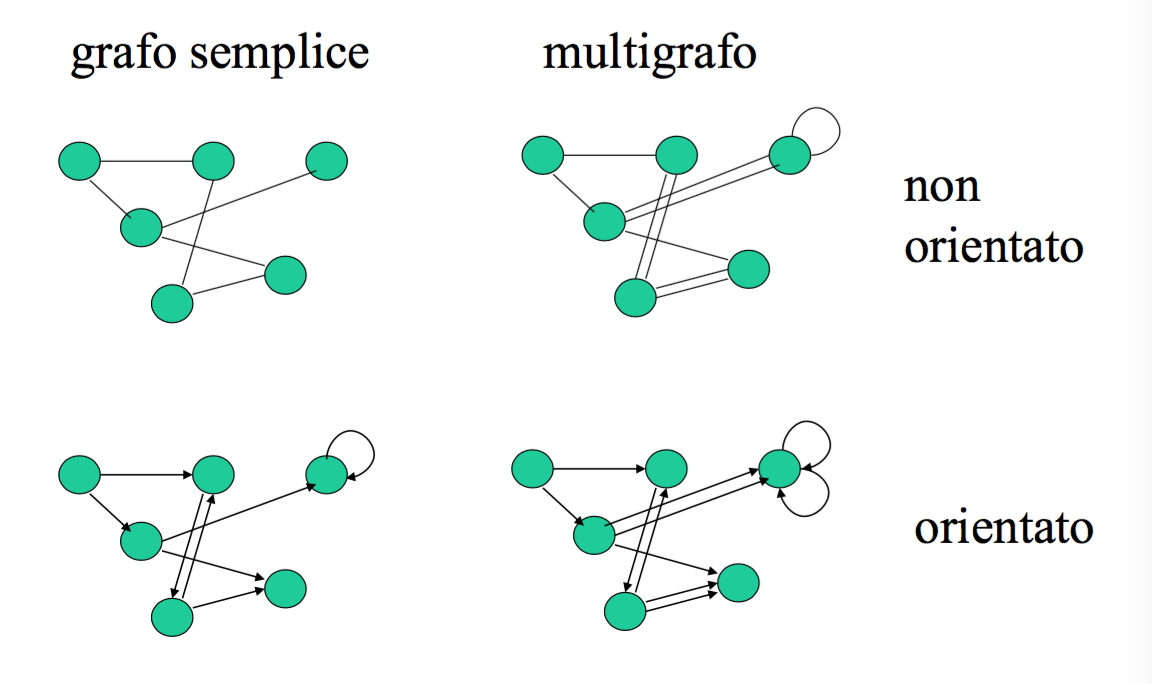
\includegraphics[width=0.75\textwidth]{./notes/immagini/l2-grafi.png}
\caption{Varie tipologie di grafi}
\end{figure}

Se un grafo è semplice, un arco può essere espresso con:

$$
e = uv \in E \text{, con } u,v \in V
$$

e si dice che l'arco \emph{e} è incidente in \emph{u} e \emph{v}. Da
notare che se il grafo è orientato
$e = uv \neq vu$ e la terminologia diventa
``l'arco \emph{e} esce da \emph{u} e entra in \emph{v}''.

Il \textbf{grado} di un vertice \emph{v} viene indicato con $\delta(v)$ e rappresenta il numero di archi incidenti in quel
vertice. Se il grafo è ordinato, il suo \textbf{grado uscente} $\delta^+(v)$ è il numero di archi uscenti e il suo \textbf{grado entrante} è $\delta^-(v)$.

Se due vertici sono collegati da un arco, questi vengono detti
\textbf{adiacenti}.

Un \textbf{cammino} di lunghezza \emph{k} da un vertice \emph{u} ad un
vertice \emph{v} in un grafo \emph{G=(V,E)}, è una sequenza di
\emph{k+1} vertici $x_0 \ldots x_k$, tali che 

$$x_0 = u$, $x_k = v$ e $x_{i-1}x_i \in E \forall i = 1\ldots k$$.

Se il cammino ha lunghezza 0, questo viene detto \textbf{nullo}, mentre
se il vertice di partenza coincide con quello di arrivo, il cammino
prende il nome di \textbf{chiuso}.

Un cammino viene detto \textbf{semplice} quanto tutti i vertici che lo
compongono sono distinti, ad eccezione del primo, che può coincidere
con l'ultimo. Un cammino semplice e il primo vertice coincide con
l'ultimo, questo prende il nome di \textbf{ciclo}. L'esempio più
semplice di ciclo è dato da un cappio.

Un grafo \textbf{aciclico} è un grafo che non contiene cicli.

Quando esiste almeno un cammino dal vertice \emph{u} al vertice
\emph{v}, si dice che \emph{v} è \textbf{accessibile} (o
\textbf{raggiungibile}) da \emph{u}. Questa definizione è simmetrica
solamente nel caso di un grafo non orientato.

Un grafo non orientato si dice \textbf{connesso} se esiste almeno un
cammino tra ogni coppia di vertici.

Le \textbf{componenti connesse} di un grafo sono le classi di
equivalenza dei suoi vertici rispetto alla relazione di accessibilità,
ovvero un sottoinsieme di vertici che sono tutti tra loro accessibili.

Nel caso di un grafo orientato, si dice che è \textbf{fortemente
connesso} se esiste almeno un cammino tra ogni vertice del grafo. In
modo analogo è possibile definire le \textbf{componenti fortemente
connesse}

Sia la \textbf{connessione} che la \textbf{connessione forte} hanno le
proprietà:

\begin{itemize}
\item
  \textbf{riflessiva}: se c'è una connessione tra \emph{u} e \emph{v},
  c'è anche tra \emph{v} e \emph{u}
\item
  \textbf{transitiva}: se c'è una connessione tra \emph{u} e \emph{v} e
  tra \emph{v} e \emph{z}, allora c'è anche tra \emph{u} e \emph{z}.
\end{itemize}

Un sotto-grafo del grafo \emph{G=(V,E)} è un grafo \emph{G' = (V', E')}
tale che:

$$
V' \subseteq V \: \text{e} \: E' \subseteq \{ uv : uv \in E \text{ e } u,v \in V' \}
$$

ovvero un grafo che ha alcuni vertici e alcuni archi del grafo iniziale.
Da notare che se tolgo un vertice, devo togliere anche tutti gli archi
incidenti in quel vertice.

Se il sotto-grafo viene ottenuto rimuovendo solo dei vertici, questo
prende il nome di \textbf{indotto}, perché la rimozione degli archi
viene forzata dalla rimozione dei vertici.

\subsection{Rappresentazione dei
grafi}\label{rappresentazione-dei-grafi}

Per rappresentare i grafi in un calcolatore è possibile utilizzare la
matrice delle adiacenze o la lista delle adiacenze.

\begin{figure}[htbp]
\centering
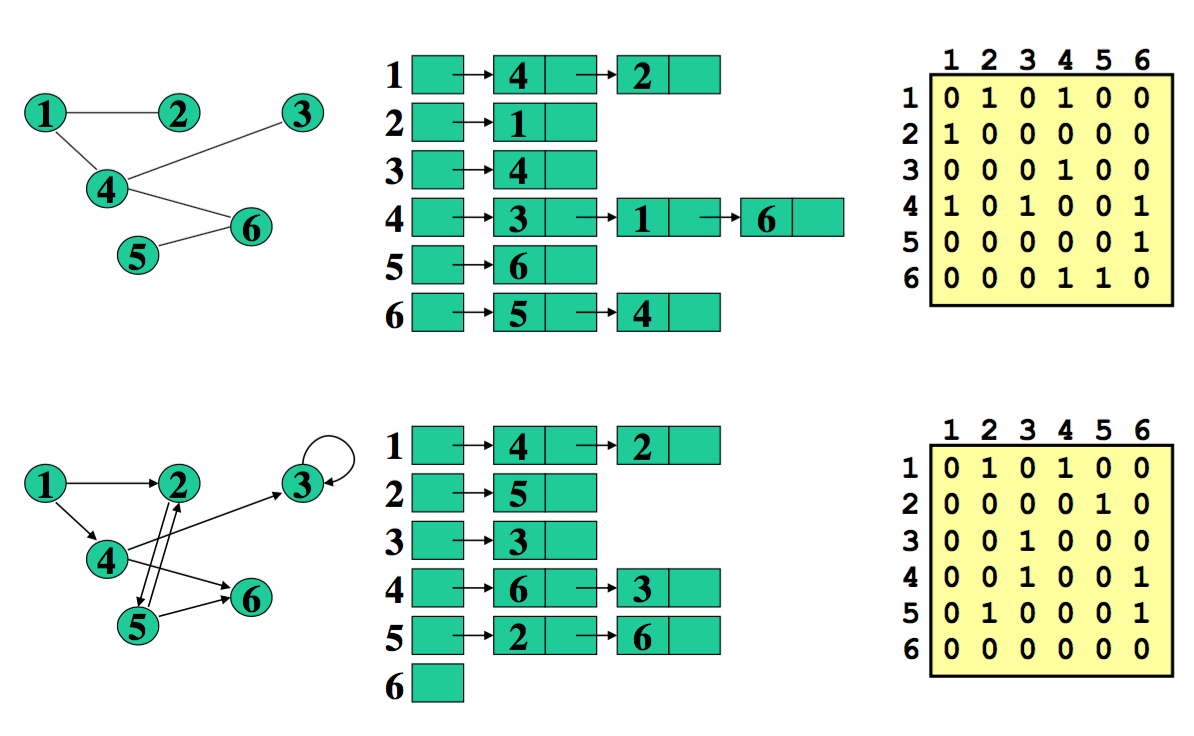
\includegraphics[width=0.75\textwidth]{./notes/immagini/l2-rappr.png}
\caption{Rappresentazione dei grafi}
\end{figure}

\subsubsection{~Lista delle adiacenze}\label{lista-delle-adiacenze}

Per ogni vertice del grafo viene tenuta in memoria una lista \textit{Adj} dei vertici
adiacenti al vertice:

$$
Adj[u] = \{v | uv \in E\} \: \forall u \in V 
$$

Questa rappresentazione richiede memoria per:

\begin{itemize}
\tightlist
\item
  \textit{n\ =\ \textbar{}V\textbar{}} puntatori alla cima delle liste
\item
  \textit{m\ =\ \textbar{}E\textbar{}} elementi per le liste (in totale)
  se il grafo orientato, se è non orientato è \textit{2m}.
\end{itemize}

\subsubsection{Matrice delle adiacenze}\label{matrice-delle-adiacenze}

Viene utilizzata una matrice booleana quadrata che tante righe e tante
colonne, quanti sono i vertici del grafo.

Ogni elemento della matrice vale 1 se i due vertici sono adiacenti, 0
altrimenti:

$$
a_{u,v} = 1 \text{ se } uv \in E
$$

Se il grafo è non orientato, la matrice delle adiacenze è simmetrica.

Il consumo di memoria è $n^2$.

Se il grafo è \textbf{sparso}, ovvero il grado dei vertici è minore del
logaritmo del numero dei vertici, la matrice delle adiacenze risulta
peggiore della rappresentazione con liste in termini di memoria
occupata.

Più formalmente, assumendo che il grafo abbia \textit{n} vertici e \textit{m} archi e che, sia i puntatori, sia gli interi, occupino 32 bit.

Si ha che la lista delle adiacenze occupa $32(n+2m)$, mentre la matrice richiede $n^2$.

La matrice risulta quindi vantaggiosa quando:

\begin{align*}
	32(n+2m) &< n^2 \\
	m &< \frac{n(n-32)}{64}
\end{align*}


\subsection{Calcolo del grafo trasposto}\label{calcolo-del-grafo-trasposto}

Dato un grafo orientato \emph{G=(V,E)} si vuole ottenere $ G^T = (V, E^T)$ in modo che gli archi siano rovesciati, ovvero $E^T = \{uv | vu \in E\}$.

Utilizzando la rappresentazione con la matrice delle adiacenze, è
necessario attraversare metà della matrice e mettere a 1 la cella
\emph{i,j} se \emph{j,i} è a 1. La complessità risulta quindi essere
$O(n^2)$.

Con la lista delle adiacenze l'algoritmo risulta essere


\begin{algorithm}
	\begin{algorithmic}[1]
		\Function{Trasponi}{$Adj,\: Adj^T,\: n$}
			\For{$v = 1 \: to \: n$}
				\State $Adj^T[v] \gets nil$
			\EndFor
			\For{$u = 1 \: to \: n$}
				\State {$x \gets Adj[u]$}
				\While{$x \neq nil$}
					\State{$v \gets x.v$}
					\State{$y \gets nodo(u, Adj^T[v])$}
					\State{$Adj^T[v] \gets y$}
				\EndWhile
			\EndFor
		\EndFunction
	\end{algorithmic}
	\caption{Trasponi: calcolo del grafo trasposto utilizzando la rappresentazione con la lista delle adiacenze}
\end{algorithm}

Ovvero viene attraversata la lista delle adiacenze del grafo originale,
e per ogni elemento delle liste, lo aggiunge ``\emph{al contrario}''
nella nuova lista delle adiacenze.

La complessità risulta quindi essere \emph{O(m+n)}, questo perché il
secondo \texttt{for} esamina tutti i possibili archi, quindi anziché
avere complessità \emph{n} (numero di vertici) ha complessità \emph{m}
(numero di archi).

\subsection{(Esercizio) Ricerca del pozzo
universale}\label{esericizio-ricerca-del-pozzo-universale}

Un vertice è un \textbf{pozzo universale} se può essere raggiunto da
tutti gli altri vertici del grafo, dal quale però non è possibile
raggiungere altri vertici.

Trovare un algoritmo che riesce a risolvere il problema in \emph{O(n)}.


\begin{verbatim}
	- Si cerca un arco tra il nodo 2 -> 1
		- se il bit è a 1, 2 non è un pozzo universale
		- si passa al successivo fino a che non si trova uno nodo che va verso 1,  ad esempio 4->1 a 0
			- in questo modo è possibile escludere il nodo 1
		- in questo modo posso partire dal k+1 in questo caso 5
			- 6->5
				se 0, escludo il 5
				se 1, escludo il 6
		- questo si ripete fino a che non rimane almeno un candidato pozzo
		- Se non c'è nessun canditato, non può esserci un pozzo
		- Se c'è un candidato è necessario verificare che sia un pozzo (forse)
		  la complessità è quindi O(n+n)
\end{verbatim}
	% !TEX encoding = UTF-8
% !TEX program = pdflatex
% !TEX root = InformationRetrieval.tex
% !TEX spellcheck = it-IT

% 6 Ottobre 2016

%\chapter{Rappresentazione dei documenti}
%\section{Analisi automatica del testo}

Tutto è iniziato quando George K. \textbf{Zipf}, uno studioso americano di linguistica ha formulato delle leggi empiriche che mettono in relazione la \textbf{frequenza di una parola} con la sua \textbf{forma} e \textbf{significato}. 
Solo in un secondo momento queste leggi sono state applicate all'indicizzazione dei documenti.

L'osservazione di partenza è stata quella che ci sono poche parole che sono veramente molto frequenti, come gli articoli, e che sono poco significative rispetto il contenuto informativo del documento. Ci sono poi tante parole poco frequenti, alcune delle quali sono fortemente correlate al contenuto informativo del documento. Il gioco è quindi quello di sfruttare al meglio tali parole.

Questo andamento può essere rappresentato graficamente, prima andando a contare le frequenze delle singole parole, per poi andare ad ordinarle da quella più frequente a quella meno frequente. La distribuzione così ottenuta è intera, ma può essere approssimata da un'iperbole.

Tipicamente in inglese:
\begin{itemize}
	\item Le due parole più frequenti sono \textit{the} e \textit{of}, mediamente sono il 10\% delle parole del documento.
	\item Le 6 parole più frequenti corrispondo a circa il 20\% delle occorrente e le 50 parole più frequenti corrispondo a circa il 40\% dei testi. Questo deriva dal fatto che la lingua deve essere ridondante in modo che sia facile da capire.
	\item Considerando un'insieme di documenti molto ampio, circa la metà delle singole parole di quel campione compare una sola volta. Queste sono parole più significative dal punto di vista dell'informazione. Tuttavia è necessario tenere conto che in questo insieme di parole possono comparire anche gli errori di battitura.
\end{itemize}

\subsection{Legge di Zipf}

La legge di Zipf afferma che dato un campione di testi e calcolata la frequenza $f$ delle parole, una volta che si sono messe le parole in ordine decrescente di frequenza, cioè si sono ordinate le parole in base al ragno \textit{r}, la distribuzione che si ottiene ha un andamento assimilabile ad una iperbole e si ha che

$$
r \times f = k
$$

ovvero la distribuzione è data da $ f = \cfrac{k}{r}$.

Se anziché ragionare in termini di frequenza assoluta si passa a considerare quella relativa, ovvero la probabilità osservata di occorrenza della parola, la legge di Zipf può essere riscritta come 

$$
r \times P_r = c
$$

Dove $P_r$ è la probabilità di occorrenza della parola che occupa il rango $r$-esimo e $c$ è una costante ($c = 0.1$ per l'inglese).

Si ha che per la lingua inglese $c \approx 0,1$ e l'iperbole che si ottiene è riportata in figura \ref{fig:zipf}

\begin{figure}[htbp]
\centering
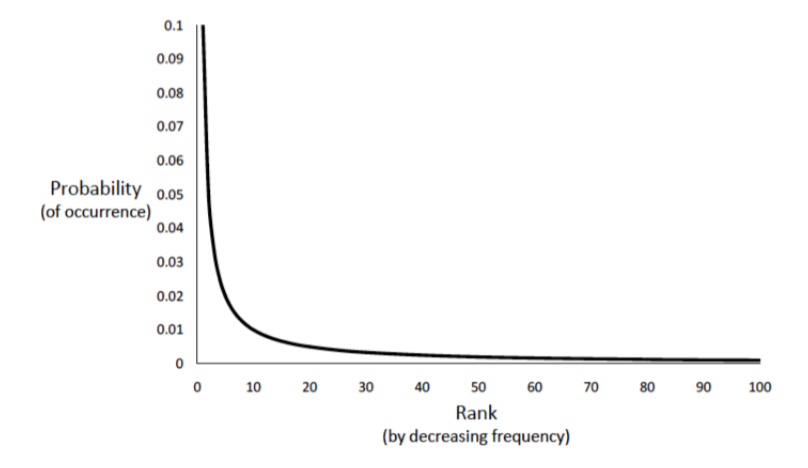
\includegraphics[width=0.55\linewidth]{images/l3-zipf}
\caption{Rango rispetto la probabilità di occorrenza assumendo valida la legge di Zipf con $c = 0.1$}\label{fig:zipf}
\end{figure}

\subsection{Indicazioni di H.P. Luhn}

L'idea per l'indicizzazione è quindi quella di definire due soglie di \textit{cut-off} per evitare di prendere in considerazione le parole troppo frequenti, perché poco significative, e quelle troppo poco, per limitare l'effetto degli errori di battitura.

Ogni parola ha un certo \textbf{resolving power}, ovvero una certa capacità di discriminare il contenuto del documento da quello degli altri e di caratterizzare il contenuto della collezione.

\begin{figure}[htbp]
	\centering
	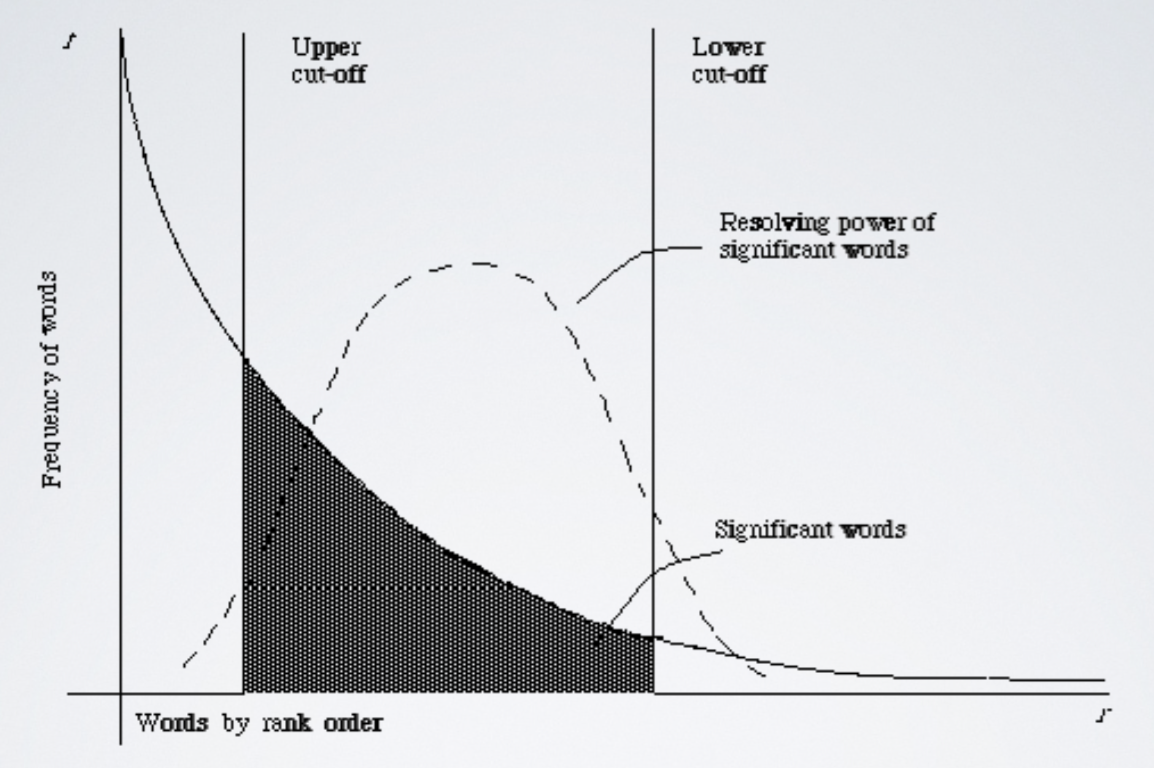
\includegraphics[width=0.55\linewidth]{images/l3-cutoff}
	\caption{Plot della curva $r \times f$ che evidenzia la posizione delle parole significative.}
\end{figure}

Questo vale per le collezioni generiche dei documenti, mentre se si parla di un argomento specifico si può dare maggiore peso a determinate parole. Ad esempio può capitare in che se viene preso in esame un manuale di MySQL è ovvio che le parole ``MySQL'' e  ``table'' compariranno tante volte anche se non sono articoli.

C'è anche un altro discorso relativo alla forma plurale, che in conteggio di frequenza vengono considerate come diverse, quando in realtà può essere che abbia lo stesso valore informativo della forma singolare. In alcuni casi è quindi opportuno sommare le occorrenze della forma plurale e di quella singolare.

Si ha quindi che i passi per applicare le indicazioni di Luhn sono:

\begin{itemize}
	\item Si calcoli la frequenza di ogni descrittore in ogni documento della collezione di riferimento. C'è inoltre da scegliere come trattare le parti di contorno dei documenti come l'indice, la premessa, ecc. tali parti tipicamente non vengono considerate.
	\item Si calcoli la frequenza totale di ogni descrittore.
	\item Si ordino i descrittori per frequenza decrescente.
	\item Si scelga una soglia di \textit{upper cut-off} e si rimuovano dalla lista i descrittori con frequenza superiore alla soglia. In questo modo si rimuovono gli articoli, le preposizioni, ecc.
	\item Si scelga un'altra soglia di \textit{lower cut-off} e si rimuovano dalla lista i descrittori con frequenza inferiore al valore di soglia. In questo modo si rimuovono i descrittori ``rumore''  o che non apportano alcun contribuito alla descrizione del contenuto.
\end{itemize}

\noindent Entrambe le soglie possono essere calcolate in modo euristico.

Le parole che vengo eliminate dalle soglie di cut-off vengono nominate \textbf{stop word} e sono raccolte nella lista che prende il nome di \textbf{stop list}.


\textbf{{\color{Red} Possibile esercizio:}} Domande relative alle osservazioni proposte da Zipf e Luhn.

\section{Indicizzazione}

L'indicizzazione ha l'obiettivo di rappresentare il contenuto informativo di un documento e nel tempo questo processo ha preso una struttura a fasi.

Il documento viene rappresentato da dei descrittori che vengono utilizzati per la costruzione degli indici, utili al reperimento dell'informazione.

Quindi l'indicizzazione fornisce automaticamente una rappresentazione più compatta e direttamente utilizzabile del contenuto informativo del documento. Gli indici sono utilizzati come surrogati del contenuto del documento durante la fase di reperimento.

L'indicizzazione può essere svolta:
\begin{itemize}
	\item manualmente
	\item in modo automatico
	\item in modo semi-automatico, quando è necessario intervenire all'interno del processo per prendere delle decisioni che non possono essere prese in modo automatico.
\end{itemize}

\noindent Tutti questi metodi funzionano estraendo direttamente dal documento le informazioni. Tuttavia possono essere estesi in modo che vengano presi in considerazione anche dei dizionari o delle meta-informazioni.

\begin{figure}[htbp]
	\centering
	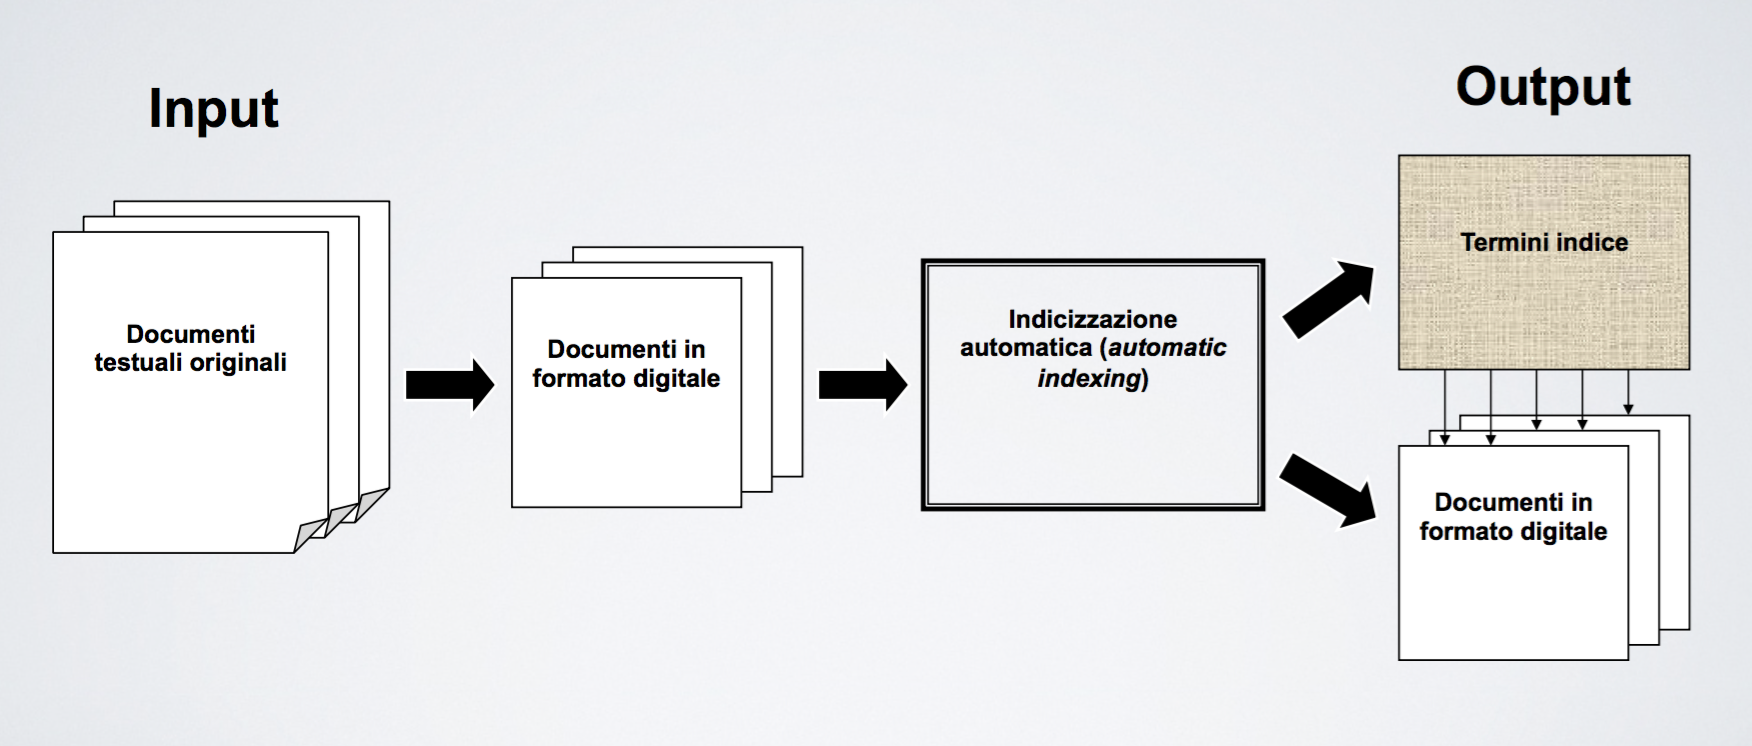
\includegraphics[width=0.7\linewidth]{images/l3-indicizzazione}
	\caption{Schema generale dell'indicizzazione}
\end{figure}

\subsection{Indicizzazione automatica dei testi}

L'indicizzazione automatica di un documento testuale è un processo che esamina automaticamente gli oggetti informativi (parole, frasi, didascalie, figure, ecc.) che compongono il documento e produce una lista di termini indice presenti nell'intera collezione dei documenti.

L'estrazione dei termini indice viene fatta da appositi algoritmi e, una volta estratti, questi vengono collegati ai diversi documenti che li contengono.
Così facendo durante il reperimento sarà sufficiente fare riferimento ai termini indice e non all'intera collezione.

\subsection{Attuazione dell'indicizzazione automatica}

L'indicizzazione automatica dei documenti testuali viene eseguita in più fasi, che devono essere attuate in sequenza:

\begin{enumerate}
	\item Analisi lessicale e selezione delle parole.
	\item Eventuale rimozione delle stop word.
	\item Riduzione delle parole originali alle rispettive radici (\textit{STEM}). Ad esempio le forme plurali vengono ridotte a quelle singolari.
	\item Composizione dei termini. Come ad esempio ``information retrieval''. Ovvero le parole vengono combinate tra loro quando si trovano ad una determinata distanza.
	\item Creazione dell'indice.
	\item Eventuale pesatura degli elementi dell'indice. 
\end{enumerate}

Alla fine di queste fasi l'indice sarà composto da parole, termini e frasi che noi riteniamo significative, assieme alle informazioni del peso che gli diamo e alla loro frequenza all'interno dei documenti.









	%\appendix
	
	%%\renewcommand{\glossaryname}{Glossario}

%\newglossaryentry{Cordova}
%{
%	name=\glslink{Cordova}{Cordova},
%	text=Cordova,
%	sort=Cordova,
%	description={Apache Cordova è un framework open source per la realizzazione di applicazioni ibride che offre delle API che permettono di accedere via JavaScript ad alcune funzionalità native del dispositivo, come l'accelerometro o la fotocamera}
%}
\subsection*{A}

\underline{\textbf{ARPA}}: %TODO

\underline{\textbf{ARPANET}}: %TODO

\underline{\textbf{Assembler}}: %TODO

\subsection*{B}

\underline{\textbf{Beowulf}}: %TODO

\subsection*{C}

\subsection*{D}

\underline{\textbf{Debian}}: %TODO

\underline{\textbf{DFSG}}: %TODO

\subsection*{E}

\subsection*{F}

\underline{\textbf{Free Software Foundation}}: %TODO

\underline{\textbf{Freeware}}: %TODO

\underline{\textbf{fsf}}: %TODO

\subsection*{G}

\underline{\textbf{GNU}}: %TODO

\underline{\textbf{GPL}}: %TODO

\subsection*{H}

\subsection*{I}

\subsection*{J}

\subsection*{K}

\underline{\textbf{Kernel}}: %TODO

\subsection*{L}

\underline{\textbf{Linux}}: %TODO

\subsection*{M}

\underline{\textbf{Mimix}}: %TODO

\underline{\textbf{MUTIX}}: %TODO

\subsection*{N}

\underline{\textbf{Netscape}}: %TODO

\underline{\textbf{nslu2}}: %TODO

\subsection*{O}

\underline{\textbf{OSI}}: %TODO

\subsection*{P}

\underline{\textbf{PDP}}: %TODO

\subsection*{Q}

\subsection*{R}

\underline{\textbf{RedHat Enterprise Linux}}: %TODO

\underline{\textbf{Routes}}: %TODO



\subsection*{S}

\underline{\textbf{StarOffice}}: %TODO

\underline{\textbf{Sun}}: 

\underline{\textbf{S\&P}}: %TODO

\underline{\textbf{Shareware}}: %TODO

\underline{\textbf{Symbolics}}: %TODO	

\subsection*{T}

\underline{\textbf{TECO}}: %TODO

\subsection*{U}

\underline{\textbf{Unix}}: %TODO

\subsection*{V}

\subsection*{W}

\subsection*{X}

\subsection*{Y}

\subsection*{Z}


	




	
	
\end{document}